%
% domain.tex -- domain for differential equation
%
% (c) 2019 Prof Dr Andreas Müller, Hochschule Rapperswil
%
\documentclass[tikz]{standalone}
\usepackage{amsmath}
\usepackage{times}
\usepackage{txfonts}
\usepackage{pgfplots}
\usepackage{csvsimple}
\usetikzlibrary{arrows,intersections,math}
\begin{document}
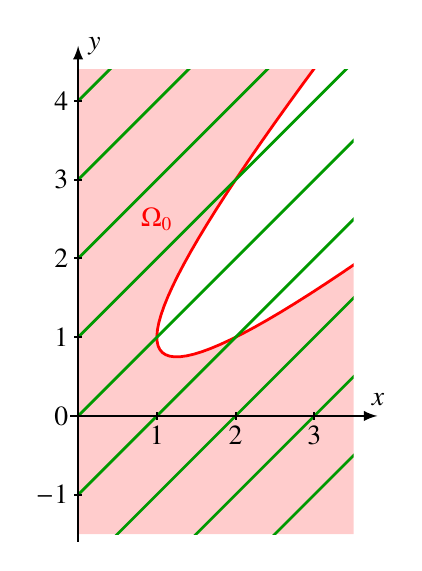
\begin{tikzpicture}[>=latex]

\definecolor{darkgreen}{rgb}{0,0.6,0}

\begin{scope}
\clip (0,-1.5) rectangle (3.5,4.4);

\fill[color=red!20] (0,-1.5)--(3.5,-1.5)--
	plot[domain=-5:2,samples=100] ({1+\x*\x},{1+\x+\x*\x})
	--(0,4.5)--cycle;

\draw[line width=1pt,color=red]
	plot[domain=-5:2,samples=100] ({1+\x*\x},{1+\x+\x*\x});

\foreach \y in {-4,...,4}{
	\draw[line width=1pt,color=darkgreen] (0,\y)--(5,{5+\y});
}

\end{scope}

\foreach \y in {-1,...,4}{
	\draw[line width=0.7pt] (-0.05,\y)--(0.05,\y);
	\node at (0,\y) [left] {$\y$};
}

\foreach \x in {1,...,3}{
	\draw[line width=0.7pt] (\x,-0.05)--(\x,0.05);
	\node at (\x,0) [below] {$\x$};
}

\draw[->,line width=0.7pt] (-0.1,0)--(3.8,0) coordinate[label={$x$}];
\draw[->,line width=0.7pt] (0,-1.6)--(0,4.7) coordinate[label={right:$y$}];

\node[color=red] at (1,2.5) {$\Omega_0$};

\end{tikzpicture}
\end{document}

